\chapter{Broadcast}

Il primo esempio di comunicazione tra processi è il \textit{broadcast}. Consideriamo un sistema distribuito dove un'entità ha una qualche informazione da condividere con tutte le altre entità. Il processo di inviare un messaggio a tutti gli altri processi è chiamato \textit{broadcast}.

Sia $\mathcal{E}$ l'insieme di tutte le entità nel sistema distribuito e sia $G = (V, E)$ il grafo che rappresenta la rete di comunicazione, dove $V = \mathcal{E}$ e $E$ è l'insieme degli archi che rappresentano le interconnessioni tra i nodi.

Prima di procedere con l'algoritmo di broadcast, è importante assumere alcune restrizioni sul sistema distribuito:
\begin{description}
    \item[Bidirectional Links (BL):] Consideriamo un grafo non diretto, dove ogni arco rappresenta una connessione bidirezionale tra due nodi.
    \item[Total Reliability (TR):] Assumiamo che i messaggi inviati tra i nodi siano sempre consegnati senza errori o perdite.
    \item[Connectivity (CN):] Il grafo $G$ è connesso, il che significa che esiste un percorso tra ogni coppia di nodi nel grafo. Questa assunzione è fondamentele per garantire la risoluzione del problema di broadcast, poiché se il grafo non fosse connesso, alcuni nodi non potrebbero ricevere il messaggio.
    \item[Unique Initiator (UI):] Supponiamo che ci sia un unico nodo che inizia il processo di broadcast, chiamato \texttt{initiator}. Questo nodo è responsabile di inviare il messaggio iniziale a tutti gli altri nodi.
\end{description}

Formalmente, il problema di broadcast può essere definito come segue: dato un grafo $G = (V, E)$ e un nodo $s \in V$ che è l'initiator, l'obiettivo è garantire che ogni nodo $v \in V$ riceva un messaggio da $s$. 

Definiamo l'insieme $\Sigma = \{\texttt{initiator}, \texttt{idle}, \texttt{informed}\}$ come l'insieme di tutti gli stati che può assumere un nodo $x \in \mathcal{E}$.

Definiamo ora le configurazioni del sistema. Una configurazione $C$ è una funzione che associa a ogni nodo $x \in \mathcal{E}$ uno stato in $\Sigma$. Inizialmente, la configurazione $C_{init}$ è tale che esiste unico nodo $s \in V$ tale che $C_{init}(s) = \texttt{initiator}$ e $C_{init}(x) = \texttt{idle}$ per ogni nodo $x \in V \setminus \{s\}$. Il numero di configurazioni iniziali possibili è
\[
    \binom{n}{1} = n,
\]
dove $n$ è il numero di nodi nel grafo. Questo perché possiamo scegliere qualsiasi nodo come initiator.

L'unica configurazione finale accettabile è quella in cui ogni nodo $x \in V$ è nello stato \texttt{informed}, ovvero
\[
    C_{final}(x) = \texttt{informed} \quad \forall x \in V.
\]

Quindi, il problema del broadcast si formalizza mediante la quadrupla:
\[
    \langle \mathcal{R},\ \Sigma,\ C_{init},\ C_{final} \rangle,
\]
dove $\mathcal{R} = \{\texttt{BL, TR, CN, UI}\}$ è l'insieme delle restrizioni, $\Sigma$ è l'insieme degli stati, $C_{init}$ è la configurazione iniziale e $C_{final}$ è la configurazione finale desiderata.

\section{Algoritmo Flooding}

L'idea generale dell'algoritmo di broadcast è quella di utilizzare un approccio di flooding, dove ogni nodo che riceve il messaggio lo inoltra a tutti i suoi vicini. L'algoritmo può essere descritto come segue:
\begin{algorithm}[H]
\caption{Algoritmo di Broadcast (Flooding)}
    \begin{algorithmic}
    \If{$C(s) = \texttt{initiator}$}
        \State $C(s) \gets \texttt{informed}$
        \ForAll{$v \in N(s)$}
            \State send($m$, $v$)
        \EndFor
    \EndIf
    \State
    \If{$C(x) = \texttt{idle}$}
        \State $m \gets$ receive() 
        \State $C(x) \gets \texttt{informed}$
        \ForAll{$v \in N(x) \setminus \{\texttt{sender}\}$}
            \State send($m$, $v$)
        \EndFor
    \EndIf
    \State
    \If{$C(x) = \texttt{informed}$}
        \State do\_nothing()
    \EndIf
    \end{algorithmic}
\end{algorithm}

Descritto in questa maniera, l'algoritmo di flooding risolve il task nella maniera corretta, e dimostreremo inoltre che termina in un tempo finito. Tuttavia, è importante notare che questo algoritmo non è efficiente in termini di complessità di messaggi, poiché ogni nodo potrebbe ricevere lo stesso messaggio più volte da diversi vicini, portando a un numero esponenziale di messaggi inviati.

\textbf{Osservazione.} Se non considerassimo l'insieme degli stati $\Sigma = \{\texttt{initiator}, \texttt{idle}\}$ e non avessimo la condizione che un nodo non inoltra il messaggio se è già informato, l'algoritmo di flooding potrebbe non terminare, poiché i nodi continuerebbero a inoltrare il messaggio indefinitamente.

\begin{lemma}
L'algoritmo di flooding termina in un tempo finito. Sia $\texttt{diam}(G)$ il diametro del grafo $G$, ovvero la massima distanza tra due nodi qualsiasi nel grafo. 

Esiste un tempo massimo $\tau$ tale che tutti i nodi $x$ a distanza $h$ da $s$ ricevano il messaggio $m$ entro il tempo $\tau$.
\[
    \forall h \leq \texttt{diam}(G),\ \exists \tau \in \mathbb{R}^{+}:\ \forall x \in V\ |\ dist(x,s) = h \implies C_{final}(x) = \texttt{informed} \land t(x) \leq \tau.
\]

\begin{proof}
Dimostriamo il lemma per induzione su $h$.
\begin{description}
    \item[Passo Base $\mathbf{h = 1}$] Sfruttando la condizione di Total Reliability, ogni nodo $v$ adiacente a $s$ riceve il messaggio $m$ entro un tempo finito $\tau_1$. Quindi, per ogni nodo $v$ tale che $dist(v, s) = 1$, abbiamo $C_f(v) = \texttt{informed}$ e $t(v) \leq \tau_1$.
    \item[Passo Induttivo $\mathbf{h + 1}$] Sfruttando la condizione di Connectivity, per ogni nodo $x \in V \setminus \{s\}:\ d(s, x) = h + 1$. 
    
    Questo implica che esiste un shortest path $P$ da $s \to x$ di lunghezza $h + 1$. Sia $y$ il nodo adiacente a $x$ su questo percorso, quindi $dist(y, s) = h$. Per ipotesi induttiva, esiste un tempo finito $\tau_h$ tale che $C_{final}(y) = \texttt{informed}$ e $t(y) \leq \tau_h$. 
    
    Sfruttando nuovamente la condizione di Total Reliability, il nodo $x$ riceve il messaggio da $y$ entro un tempo finito $\tau_{h+1}$, quindi $C_{final}(x) = \texttt{informed}$ e $t(x) \leq \tau_{h+1}$.
\end{description}
\end{proof}

\end{lemma}

\begin{lemma}[Message Complexity]
    L'algoritmo di flooding ha una message complexity 
    \[
        M[\texttt{Flooding}] = \theta(|E|) = \theta(m).
    \]
    \begin{proof}
        Dimostriamo il lemma utilizzando due metodi differenti. Nel primo metodo facciamo un'analisi diretta del numero di messaggi inviati, mentre nel secondo metodo utilizziamo un'analisi basata sui nodi e sui loro vicini.
        \begin{description}
            \item[Metodo I: ] L'idea è di contare il numero di messaggi che attraversano un arco. Se $state(s) = \texttt{initiator}$, il numero di messaggi che passano attraverso i suoi archi incidenti è esattamento $1$, ossia solo il messaggio $m$ da inoltrare. Consideriamo adesso due nodi $x \neq s$ e $y \neq s$ adiacenti e contiamo il numero di messaggi che passano attraverso l'arco $(x, y)$. Siano $t_x$ e $t_y$ gli istanti di tempo in cui $x$ e $y$ ricevono il messaggio $m$, e consideriamo il caso in cui $t_x < t_y$. In questo caso, $x$ inoltra il messaggio $m$ a $y$. Tuttavia, al tempo $t_y$, $y$ riceve una copia del messaggio da un nodo $z \neq x$ un'istante prima di riceverlo da $x$. In questo caso, $y$ inoltra il messaggio a $x$. Quindi, il numero massimo di messaggi che passano attraverso l'arco $(x, y)$ è $2$. Quindi ogni arco può essere attraversato da al massimo $2$ messaggi, dimostrando che $M[\texttt{Flooding}] = \theta(2|E|) = \theta(m)$.
            \item[Metodo II: ] Una dimostrazione più precisa può essere ottenuta considerando il numero di messaggi inviati da ogni nodo. Se $state(s) = \texttt{initiator}$, il numero di messaggi inviati è esattamente $d(s)$ dove $d(x) = N(x)$ è il grado di $x$. Consideriamo adesso un nodo $x \neq s$. Il numero di messaggi che invia è $d(x) - 1$, poiché non inoltra il messaggio al nodo da cui lo ha ricevuto. Quindi, il numero totale di messaggi inviati è
            \begin{align*}
                M[\texttt{Flooding}] &= d(s) + \sum_{x \neq s} (d(x) - 1) \\ 
                &= \sum_{x \in V} d(x) - \sum_{x \in V \setminus \{s\}} (n - 1) \\
                &= 2|E| - (n - 1) = 2m - n + 1 = \theta(m).
            \end{align*}
        \end{description}
    \end{proof}
    \textbf{Osservazione.} La somma degli gradi di tutti i nodi in un grafo è pari a $2|E|$, poiché ogni arco contribuisce al grado di due nodi.
\end{lemma}

\subsection{Complessità Temporale}

In generale, non ha senso calcolare la complessità temporale di un algoritmo in un sistema asincronom a causa dell'impossibilità di poter predire i tempo di trasmissione dei messaggi. Tuttavia, se assumiamo un sistema sincrono, ossia assumiamo \textbf{clock sincronizzati} e \textbf{bounded delay}, possiamo calcolare la complessità temporale dell'algoritmo di flooding. Assumiamo che i messaggi vengano trasmessi con un delay di $\delta$ (normalizzando, $\delta = 1$). Chiaramente, il messaggio inviato dall'initiator $s$ deve raggiungere ogni nodo $x$ a distanza $h$ da $s$ entro un tempo finito, e il tempo necessario per raggiungere il nodo più lontano da $s$ è dato \textbf{eccentricity} di $s$, che è definita come
\[
    ecc(s) = \max_{x \in V} dist(s, x).
\]
Allora, nel caso peggiore, il tempo necessario per raggiungere ogni nodo è dato dal diametro del grafo $\texttt{diam}(G)$, che è definito come
\[
    \texttt{diam}(G) = ecc(s).
\]
In conclusione, la complessità temporale \textit{ideale} dell'algoritmo di flooding è
\[
    T[\texttt{Flooding}] = \max_{x \in V} dist(s, x) \leq \texttt{diam}(G) \leq n - 1 = O(n).
\]
Si vuole dimostrare inoltre che tale protocollo sia ottimali in termini di complessità temporale, ossia che non esiste un protocollo di broadcast che possa raggiungere ogni nodo in un tempo minore del diametro del grafo. È necessario quindi dare una delimitazione inferiore alla complessità temporale di qualsiasi protocollo di broadcast. Si osserva che ciascuna entità $x$ a distanza $h$ da $s$ non può ricevere il messaggio $m$ prima di $h$ unità di tempo, poiché il messaggio deve attraversare almeno $h$ archi per raggiungere $x$. Quindi, la complessità temporale di qualsiasi protocollo di broadcast è limitata inferiormente da
\[
    T[\texttt{Broadcast}] \geq \max_{x \in V} dist(s, x) = ecc(s) \leq \texttt{diam}(G).
\]
Di conseguenza, l'algoritmo di flooding è ottimale in termini di complessità temporale, in particolare l'ideal time complexity è $T[\texttt{Flooding}] = \theta(\texttt{diam}(G))$.

\subsection{Stati ed Eventi}

Nel mondo centralizzato, dato uno stesso input ad un algoritmo deterministico, esso non solo genera lo stesso output, ma la sequenza di azioni che svolge per raggiungere tale output è sempre la stessa, ad ogni esecuzione.
Questo dettaglio non vale nel mondo distribuito. Ad esempio nel protocollo flooding, dato che il ritardo dei messaggi varia in modo indeterminato, la sequenza di azioni verso l'unica configurazione finale varia ad ogni esecuzione, anche a fronte di una stessa configurazione iniziale (cioè esecuzioni dallo stesso iniziatore). Naturalmente, per la correttezza del protocollo, una qualsiasi sequenza di azioni anche se diversa converge verso la configurazione finale.

Consideriamo il seguento grafo $G$ con $n = 3$ nodi e $m = 3$ archi, dove $x$ è l'initiator:
\begin{center}
    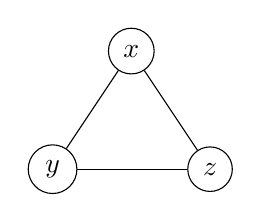
\begin{tikzpicture}
        \node[circle, draw] (x) at (1, 1.5) {$x$};
        \node[circle, draw] (y) at (0, 0) {$y$};
        \node[circle, draw] (z) at (2, 0) {$z$};
        \draw (x) -- (y);
        \draw (y) -- (z);
        \draw (z) -- (x);
    \end{tikzpicture}
\end{center}

Eseguendo una prima volta il protocollo, supponiamo che $z$ riceva il messaggio da $x$ prima di $y$.

\begin{figure}[ht!]
    \centering
    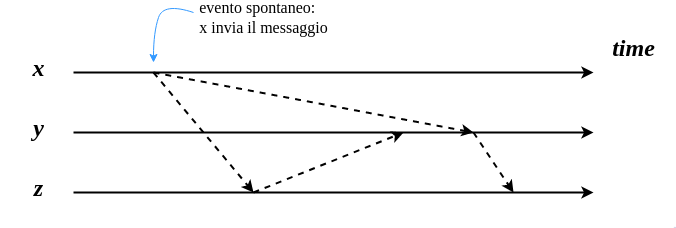
\includegraphics[width=0.6\linewidth]{images/seq1.png}
    \caption{Sequenza di azioni del protocollo di flooding, con $z$ che riceve il messaggio da $x$ prima di $y$.}
    \label{fig:seq1}
\end{figure}

Tale esecuzione può essere rappresentata mediante il seguente grafo, dove ogni nodo rappresenta una configurazione del sistema e ogni arco rappresenta un evento (cioè, l'invio o la ricezione di un messaggio). In questo caso, la sequenza di azioni è $x \to z \to y$.

\begin{center}
    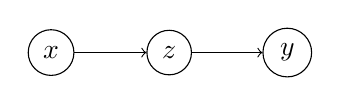
\begin{tikzpicture}
        \node[circle, draw] (x) at (1.5, 0) {$x$};
        \node[circle, draw] (z) at (3, 0) {$z$};
        \node[circle, draw] (y) at (4.5, 0) {$y$};
        \draw[->] (x) -- (z);
        \draw[->] (z) -- (y);
    \end{tikzpicture}
\end{center}

Eseguendo una seconda volta il protocollo, potrebbe capitare che i ritardi sugli archi $(x,z)$ e $(z,y)$ siano simili. Perciò, una possibile sequenza di azione potrebbe essere:

\begin{figure}[ht!]
    \centering
    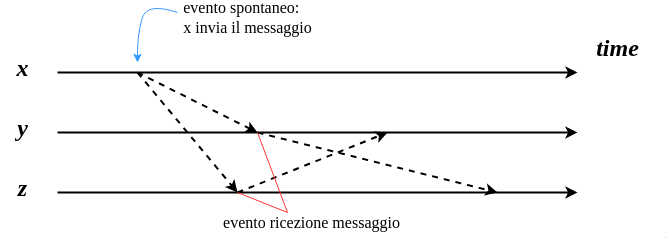
\includegraphics[width=0.6\linewidth]{images/seq2.png}
    \caption{Esecuzione del protocollo con ritardi simili sugli archi $(x,z)$ e $(z,y)$.}
    \label{fig:seq2}
\end{figure}

Tale esecuzione può essere rappresentata mediante il seguente grafo,

\begin{center}
    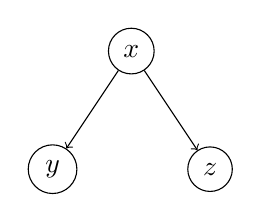
\begin{tikzpicture}
        \node[circle, draw] (x) at (1, 1.5) {$x$};
        \node[circle, draw] (y) at (0, 0) {$y$};
        \node[circle, draw] (z) at (2, 0) {$z$};
        \draw[->] (x) -- (y);
        \draw[->] (x) -- (z);
    \end{tikzpicture}
\end{center}

Dato che il grafo di comunicazione è sostanzialmente un albero ricoprente, ci sono quindi $O(n^n)$ possibili sequenze di trasmissioni (o \textbf{traiettorie}) che portano alla configurazione finale, anche a fronte di una stessa configurazione iniziale.

\subsection{Lowerbound alla Message Complexity}

\begin{definizione}[Stato Locale Interno]
    Definiamo $\sigma(x, t)$ come lo stato locale interno del nodo $x$ al tempo $t$. Di conseguenza $$\Sigma(t) = \{\sigma(x, t) :\ x \in \mathcal{E} \}$$ è l'insieme di tutti gli stati locali dei nodi al tempo $t$.
\end{definizione}
Consideriamo adesso due ambienti \textit{(environments)} $E_1$ e $E_2$ dove, lo stato interno di $x$ al tempo $t$ è lo stesso, ossia $\sigma_1(x, t) = \sigma_2(x, t)$. Allora $x$ non è in grado di \textit{distinguere} tra i due ambienti. Di conseguenza, se avviene lo stesso evento in entrambi gli ambienti, $x$ esegue la stessa azione in entrambi gli ambienti.

Segueno due proprietà fondamentali che ci permettono di dimostrare un lowerbound alla message complexity di qualsiasi protocollo di broadcast.
\begin{description}
    \item[Proprietà 1:] Se $x$ si trova in due ambienti $E_1$ e $E_2$, e lo stato interno di $x$ è lo stesso in entrambi gli ambienti al tempo $t$ ($\sigma_1(x, t) = \sigma_2(x, t)$), allora $x$ non è in grado di distinguere tra i due ambienti.
    \item[Proprietà 2:] Se due nodi distinti $x$ e $y$ ad un certo istante $t$ si trovano nello stesso stato interno ($\sigma(x, t) = \sigma(y, t)$), allora se vengono sollecitati dallo stesso evento, eseguiranno la stessa azione.
\end{description}

\begin{teorema}[Lower Bound]
    Sotto le ipotesi
    \[
    R = \{\texttt{BL, TR, CN, UI}\} 
    \]
    (ossia, bidirectional links, total reliability, connectivity e unique initiator), qualsiasi protocollo di broadcast ha una message complexity $M[\texttt{Broadcast}] = \Omega(m)$.
    \begin{proof}
        Supponiamo per assurdo che esista un protocollo di broadcast con una message complexity $M[\texttt{Broadcast}] = o(m)$ (per esempio $m-1$ messaggi). Consideriamo un grafo $G = (V, E)$, e sia $s$ l'initiator. Poiché il protocollo ha una message complexity sublineare, esiste almeno un arco $e = (x, y) \in E$ che non viene attraversato da alcun messaggio durante l'esecuzione del protocollo. Sia ora $G' = (V', E')$ costruito a partire da $G$ rimuovendo l'arco $e$ e aggiungengo un nuovo nodo $z$ tale per cui $state(z) = \texttt{idle}$ connesso a $x$ e $y$ mediante due nuovi archi, ossia
        \[
        V' = V \cup \{z\}, \quad E' = E \setminus \{e\} \cup \{(x, z), (y, z)\}.
        \]
        Siano quindi $E_1$ e $E_2$ i due ambienti, dove in $E_1$ il protocollo viene eseguito su $G$, mentre in $E_2$ il protocollo viene eseguito su $G'$.
        Le etichette degli archi in $G$ e $G'$ sono le stesse, quindi $x$ e $y$ non sono in grado di distinguere tra i due ambienti. 
        \[
            \lambda_x(x, y) = \lambda_x(x, z), \quad \lambda_y(y, x) = \lambda_y(y, z).
        \]
        \begin{figure}[ht!]
            \centering
            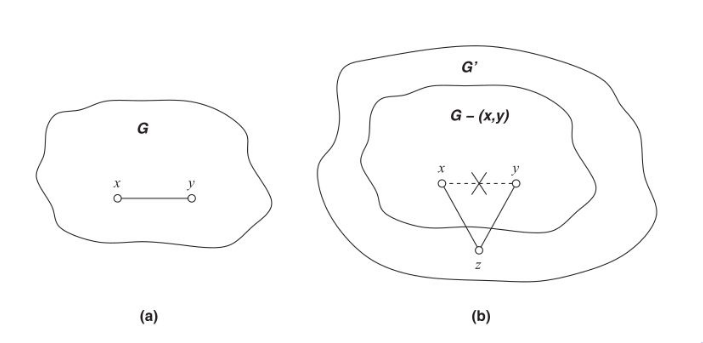
\includegraphics[width=0.8\linewidth]{images/lowerbound.png}
            \caption{Costruzione del grafo $G'$ a partire da $G$.}
            \label{fig:lowerbound}
        \end{figure}
        Allora sapendo che $x$ e $y$ non sono in grado di distinguere (\textbf{Proprietà 1}) tra i due ambienti, se viene sollecitato lo stesso evento in entrambi gli ambienti, $x$ e $y$ eseguono la stessa azione (\textbf{Proprietà 2}). Poiché in $E_1$ non inoltrano il messaggio sul arco $(x, y)$, in $E_2$ non inoltrano il messaggio né su $(x, z)$ né su $(y, z)$. Di conseguenza, il nodo $z$ non riceve mai il messaggio (poiché è collegato solo a $x$ e $y$), e quindi il protocollo di broadcast fallisce in $E_2$, portando ad una contraddizione, ossia vengono inviati $o(m)$ messaggi e rimane un nodo non raggiungibile.
    \end{proof}
\end{teorema}

\textbf{Osservazione.}
Se consideriamo una fase di preprocessing, ossia una fase iniziale in cui i nodi possono scambiarsi messaggi per costruire una mappa della rete (uno \textbf{spanning tree}), allora è possibile progettare un protocollo di broadcast con una message complexity $M[\texttt{Broadcast}] = O(n)$, che è ottimale in quanto ogni nodo deve ricevere almeno un messaggio. Tuttavia, in questo caso, la message complexity totale del protocollo (preprocessing + broadcast) è $M[\texttt{Total}] = O(n + m) = O(m)$, che è ancora ottimale in quanto ogni arco deve essere attraversato da almeno un messaggio durante la fase di preprocessing.

